\documentclass{article}
\usepackage[T1]{fontenc}
\usepackage[utf8]{inputenc}

\usepackage{xspace}
\usepackage{graphicx}
\usepackage{amsmath}
\usepackage{amsfonts}
\usepackage{subfig}
\usepackage{fullpage}
\usepackage{url,paralist}
\usepackage{caption}

\author{Philip Pickering\\ \url{pgpick@gmx.at} \and Marco Eilers\\ \url{eilers.marco@googlemail.com} \and Thomas Bracht Laumann Jespersen\\ \url{ntl316@alumni.ku.dk}}
\title{Statistical Methods for Machine Learning\\ Assignment 2: Basic Learning Algorithms}
\date{}

\newcommand{\vect}[1]{\ensuremath{\boldsymbol{\mathbf{#1}}}\xspace}

%% For readability in question 1.3
\newcommand{\Target}{\vect{\mathsf{T}}}
\newcommand{\vPhi}{\vect{\Phi}}
\newcommand{\vw}{\vect{w}}
\newcommand{\Szero}{\vect{S}_0}
\newcommand{\mzero}{\vect{m}_0}
\newcommand{\target}{\vect{\mathsf{t}}}

\newcommand{\knollA}{\textsc{knollA}\xspace}
\newcommand{\knollB}{\textsc{knollB}\xspace}
\newcommand{\knollC}{\textsc{knollC}\xspace}

%% %% Uncomment these lines to get a box around all figures
%% \usepackage{float}
%% \floatstyle{boxed}
%% \restylefloat{figure}

\begin{document}
\maketitle

\section{Neural Networks}

\begin{enumerate}\setlength{\itemsep}{-3pt}
  \item How to represent the neural network in MATLAB? One method
    could be $M\times M$ matrix (where $M$ is the number of
    neurons). Call it \vect{NN}. Then we number the neurons from
    $1,\dots,M$ and $\vect{NN}(i;j) = w_{i,j}$
\end{enumerate}

Implement a multi-layer neural network with linear output neuron and a
single hidden layer with non-linear neuron. All neurons should have
bias (offset) parameters.

To find the derivative of the activation function:
\[
\sigma(u) = \frac{|u|}{1 + |u|}
\]
we apply the quotient rule for differantiation:
\[
\frac{d}{du}\frac{f(x)}{g(x)} = \frac{g(x)f'(x) - g'(x)f(x)}{\left[g(x)\right]^2}
\]
where, in our case $f(u) = |u|$ and $g(u) = 1 + |u|$.
\begin{align}
  \frac{d}{du}\left(\frac{|u|}{1 + |u|}\right) &= \frac{(1 + |u|)\cdot 1 - (0 + 1)|u|}{(1 + |u|)^2}\\
  &= \frac{1 + |u| - |u|}{(1 + |u|)^2}\\
  &= \frac{1}{(1 + |u|)^2}
\end{align}

Implement backpropagation to compute gradient of error with respect to
the network parameters.

\section{Support Vector Machines}

\subsection{Model Selection}
Description (we normalized the data, then used the builtin function of libsvm, tried these values for gamma: [])

Result: best parameters are:

Applied to the testdata, this gives the following results:

\begin{figure}
  \includegraphics[width=\textwidth]{Code/freeBoundedSVs.eps}
  \caption{\texttt{knollC-train200} trained SVM model. Bounded support vectors are circled in green and free support vectors are circled in black.}
\end{figure}

\end{document}
